\documentclass[a4paper,10pt]{article}
\usepackage[utf8]{inputenc}
\usepackage{graphicx}        % standard LaTeX graphics tool
\usepackage{amsmath}

\DeclareMathOperator{\E}{\mathbb{E}}
% Title Page
\title{Notes on Quaternion-based EKF Orientation Estimation for a Mobile Phone }
\author{Jorhabib Eljaik Gomez}
\date{}


\begin{document}
\maketitle

% \chapter*{Quaternion-based Methods for Orientation Estimation.}
% \label{chap:methods}

\section{Initial Considerations}
In all of the followig versions of the filter, we will assume the following:

\begin{itemize}
 \item The process to be estimated is random and can be modeled as:
 $x_{k+1} = \phi_k x_k + w_k$.
 \item The measurement (observation) of the process respects the linear relationship $z_k = H_k x_k + v_k$.
 \item An initial estimate of the process at some time $t_k$ is available. This prior estimate is denoted $\hat{x}^{-}_k$.
 \item  The error covariance matrix associated with $\hat{x}^{-}_k$ is known, which corresponds to $P^{-}_k = E[e^{-}_k {e^{-}}^T_k]$ where $e^{-}_k$ is the \textbf{estimation error} defined as ${e^{-}}_k = x_k - \hat{x}^{-}_k$.
\end{itemize}

Where:
\begin{list}{variables}{}
 \item $x_k (n \times 1)$ process state vector at time $t_k$
 \item $\phi_k (n \times n)$ matrix relating $x_k$ to $x_{k+1}$ in the absence of a forcing function (no input).
 \item $w_k (n \times 1)$ noise vector with known covariance structure.
 \item $z_k (m \times 1)$ vector measurement at time $t_k$
 \item $H_k (m \times 1)$ matrix giving the (noiseless) linear relationship between the measurement and the state vector at time $t_k$
 \item $v_k (m \times 1)$ measurement error
\end{list}

Covariance matrices for the $w_k$ and $v_k$ vectors at time $t_k$ are given by $Q_k$ and $R_k$.

\subsection{Kalman Filter}
\label{sec:KalmanFilter}
Here goes a summarized explanation of the Kalman Filter.
\begin{figure}[!ht]
 \centering
 \includegraphics[width=0.5\textwidth]{./fig/kalman_loop.png}
 % kalman_loop.png: 1157x570 pixel, 72dpi, 40.82x20.11 cm, bb=0 0 1157 570
 \caption{Kalman filter algorithm. Extracted from Introduction to Random Signals and Applied Kalman Filtering.}
 \label{fig:kalmanLoop}
\end{figure}

\subsection{Sensors Calibration}
This is a very delicate and important issue that needs to be addressed. Good summarized information can be found in \cite{Cucu2012} and the selected choice described here.

\section{Simplified Version (Gyroscope and Accelerometer)}
In this simplified version we have the following description of the process:
\begin{itemize}
 \item \textbf{State Space Model:} The state is the orientation of the sensor local frame \cal{\{S\}} with respect to the earth-fixed world reference frame \cal{\{W\}} corresponding to the east-north-up system (y-axis pointing north, z-axis pointing up). This orientation is what we want to estimate, and to do so, we will use the angular velocity provided by the gyroscope as input to the system, while the measurement equation will come from the model of the accelerometer such that:

\begin{align}
 x_k &= q^w_{s_k} \\
 u_k &= \omega^s_k \\
 z_k &= f(a^s_{k})
\end{align}

In the previous equations $q^w_{s_k}$ stands for the quaternion in $rad$ at time $k$, representing the orientation between the sensor and the world reference frame (quaternions in this document have the following structure: $q = [q_{\text{real}} \quad q_{\text{vec}}]$), $\omega^s_k$ the angular velocity in $rad/s$ in the sensor reference frame while $f(a^s_{k})$ is actually the rotated gravity acceleration in \{W\} felt by the accelerometer in $m/s^2$. Recall that the accelerometer measures the acceleration acting \textbf{on} itself in its local reference frame \{S\}. We will assume also that the gravity acceleration \textbf{felt} by the accelerometer at rest in \{W\} is constant and equal to $g^w = [0 \quad 0 \quad 9.81]^T$ and that the body does not move too fast. 

\begin{figure}[h]
 \centering
 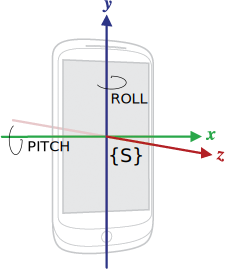
\includegraphics[width=0.4\textwidth]{./fig/axis_device.png}
 % axis_device.png: 225x269 pixel, 90dpi, 6.35x7.59 cm, bb=0 0 180 215
 \label{fig:phone_frame}
 \caption{Local sensor frame \{S\}}
\end{figure}


\item \textbf{System Dynamics:} Since our state vector consists only of the quaternion $q^w_{s_k}$, its dynamics are given by the derivate of the quaternion, i.e. $\dot{q}^w_s = \frac{1}{2}\Omega(\omega^s)q^w_s$ in continuous time. Assuming that the angular velocity remains constant over the integration time, the previus equation can be transformed into a discretized update equation of the form $q^w_{s_{k+1}} = \Phi_k q^w_{s_k}$ where $\Phi_k = e^{F\Delta T}$ and $F$ the transition matrix $\frac{1}{2}\Omega(\omega^s)$. Including the gyro noise $w$ with probability distribution $\cal{N}$ $(0,Q_c)$ and following a Taylor series expansion we get:

\begin{align}
 q^w_{s_{k+1}} &= e^{\frac{1}{2}\Omega(\omega^s_k + w_k)\Delta T} q^w_{s_k} \\
         &= (I_{4\times 4} + \frac{1}{2}\Omega(\omega^s_k)\Delta T)q^w_{s_k} + \frac{\Delta T}{2}\Xi(q^w_{s_k})w_k
\end{align}

Where the operators $\Omega$ and $\Xi$ are:

\begin{equation}
 \Omega(\omega^s_k) = \left[\begin{matrix}
                      0	        &  -(\omega^s_k)^T\\
                   \omega^s_k   &  -S(\omega^s_k)
z                  \end{matrix}\right]
\end{equation}

\begin{equation} 
 \Xi(q^w_{s_k}) = \left[\begin{matrix}
                   [-q^w_{s_k}]^T_{vec} \\
                    [q^w_{s_k}]_{real} I_{3\times3} + S([q^w_{s_k}]_{vec})
                  \end{matrix}\right]
\end{equation}

$\Delta T = t_{k+1} - t_k$ and $S(v)$ is the skew symmetric operator:

\begin{equation}
 S(v) = \left[\begin{matrix}
               0    &  -v_z  &   v_y\\
               v_z  &   0    &  -v_x\\
              -v_y  &   v_x  &    0 
              \end{matrix}\right]
\end{equation}



\item \textbf{Sensor Fusion Model: } Let us recall the discrete Kalman filter structure given by the process and sensor equations as:
\begin{align}
 x_{k+1} &= \phi_k x_k + w_k\\
 z_k     &= H_k x_k + v_k
\end{align}

Given the system dynamics previously described, the continuous state model was:
\begin{equation}
  \dot{x} = \underbrace{\frac{1}{2} S(\omega_k + w_k)}_{F} x
\end{equation}

Where $F$ is the transition matrix. 

The accelerometer can be modeled using the following equation,

\begin{equation}
 y_{k_a} = Q^T(q_k)(g^o + F_k) + v^a_k
\end{equation}

Where $g^0$ is the nominal gravity vector and measurement noise $v^a_k$

While the magnetometer can be modeled using the following equation,

\begin{equation}
 y_{k_m} = Q^T(q_k)m^0 + v^m_k
\end{equation}

Where $m^0$ is the earth magnetic field in world coordinates, or nominal magnetic field and given by $m^0 = (0 \quad \sqrt{m^2_x + m^2_y} \quad m_z)^T$

Then, following discretization the Kalman model can be written as:
\begin{align}
 x_{k+1} &= \underbrace{\left(I + \frac{1}{2}S(\omega_k)\Delta T\right)}_{\phi_k} x_k + \underbrace{\frac{\Delta T}{2}\bar{S}(q_k)w_k }_{w'_k}\\ 
 z_{k}   &=  Q^T(q_k)(g^o + F_k) + v^a_k
\end{align}

This equation is also known as the Zeroth Order Quaternion Integrator, which assumes constant angular velocity over the integration period $\Delta T$. A very detailed derivation can be found in Section 1.6.1 in \cite{Trawny2005}.

The measurement model contains so far only the accelerometer. Also, assuming quaternions of the form $q = [q_{real} \quad q_x \quad q_y \quad q_z]^T$. 

\begin{equation}
 S(\omega) = \left[
 \begin{matrix}
  0 	   & -\omega_x & -\omega_y & -\omega_z\\
  \omega_x & 0	       &  \omega_z & -\omega_y\\
  \omega_y & -\omega_z &  0	   &  \omega_x\\
  \omega_z &  \omega_y & -\omega_x &  0
 \end{matrix}\right]
\end{equation}

and 

\begin{equation}
 \bar{S}(q) = \left[
 \begin{matrix}
  -q_1 & -q_2 & -q_3 \\
   q_0 & -q_3 &  q_2 \\
   q_3 &  q_0 & -q_1 \\
  -q_2 &  q_1 &  q_0
 \end{matrix}\right]
\end{equation}

Where $F_k$ will be assumed to be zero. The measurement equation however must be linearized! Once linearized, we can obtain also $H_k$. The measurement equation for the accelerometer can be linearized by taking its Jacobian and evaluating at the most recent estimate. However, as done in \cite{Ligorio2013}, the linearized measurement matrix $H_k$ can be obtained as:

\begin{align}
 H_k = \Psi(q_k, g^0) &= \frac{\partial}{\partial q_k}  \left( q_k \otimes \bar{g}^0 \otimes q^{-1}_k \right)\\
                      &= \bar{S}_R(q_k) \bar{S}_R(g^0)^T + \bar{S}^T_L(q_k) \bar{S}_L(g^0)^T \left[\begin{matrix} -I_3 & 0 \\0  & 1 
			     \end{matrix}\right]
\end{align}

Where

\begin{equation}
 S_L = \left[\begin{matrix}
	       q_4 &  q_3 & -q_2 & q_1\\
	      -q_3 &  q_4 &  q_1 & q_2\\
	       q_2 & -q_1 &  q_4 & q_3\\
	      -q_1 & -q_2 & -q_3 & q_4
	     \end{matrix}\right]
\end{equation}

\begin{equation}
  S_R = \left[\begin{matrix}
	       q_4 & -q_3 &  q_2 & q_1\\
	       q_3 &  q_4 & -q_1 & q_2\\
	      -q_2 &  q_1 &  q_4 & q_3\\
	      -q_1 & -q_2 & -q_3 & q_4
	     \end{matrix}\right]
\end{equation}

And corresponding measurement noise covariance matrix 
\begin{equation}
 R_k = \Sigma_a
\end{equation}

Where $\Sigma_a = I_4 \sigma_v^2$.

In this way, we finally obtain the linearized measurement equations such that
\begin{equation}
 z_k = H_k q_k 
\end{equation}


There is also another possibility, which consists in using accelerometer and magnetometer readings as inputs to the QUEST \cite{Shuster1981} algorithm to produce what will be called the \emph{computed quaternion} which is then presented to the Kalman Filter as measurements, greatly simplifying its implementation \cite{Shuster1981}. A method using QUEST will be presented later in Section \ref{sect:questSection}. 

NOTE: DON'T FORGET TO CHECK THAT ALL THE QUATERNION FUNCTIONS THAT I'M USING CONSIDER THE QUATERNION IN THE SAME WAY. THE REAL PART COULD BE AT THE BEGINNING OR AT THE END OF THE VECTOR. 


\end{itemize}

\section{Estimating Orientation and Gyro Bias}

\section{Simplified Version Using the QUaternionESTimator algorithm (QUEST)}
\label{sect:questSection}
An alternative to the linearization of the accelerometer measurement equation is that of fusing the accelerometer and magnetometer measurement into a single one through an efficient statistical attitude determination method called QUEST, which stands for QUaternion ESTimator. The basic idea is that if two orientation observations are available, this information can be joint together using a statistical method. Suppose we have a set of of $N$ unit vectors $\hat{z}_k$, for which we have the mathematical model	 that relates their sensor measurement in the inertial ${i}$ frame to the body frame ${b}$ through a rotation matrix $R^b_i$ as:

\begin{equation}
 z_{kb} = R^b_i z_{ki}
\end{equation}

This set of equations is overdetermined when having two or more readings. For this reason, we want to find a solution for $R^b_i$ that minimizes the overall error for all vectors. The classical way to state this problem is as an optimization one that minimizes the sum of the squared errors for each vector measurement. Thus, the loss function can be expressed as:

\begin{equation}
 J(R^b_i) = \frac{1}{2}  \sum^{N}_{k=1}  w_k \left| z_{kb} - R^b_i z_{ki} \right|^2 
\end{equation}

Where $J$ is the loss function to be minimized, $k$ is the index for observations (measurements) $z_{k}$ is the $kth$ vector being measured, $z_{kb}$ is the matrix of measured components in the body frame and $z_{ki}$ the matrix of components in the inertial frame \cite{HallNotes2003}. The previous loss function is also known in literature as Wahba's loss function. 

Depending on how noisy measurements are, the harder it becomes to minimize this loss function. 

QUEST is just one efficient way to perform this minimization and will be described next. Many spacecraft attitude systems use this method to fuse the unit vector giving the direction to the sun or a star and the unit vector in the direction of the Earth's magnetic field. In this particular implementation we intend to do the same, with the gravity vector given by the accelerometer and the Earth's magnetic field direction provided by the magnetometer.

\subsection{QUEST}

\section{Multiplicative Kalman Filter}
The Kalman Filter explained in Section \ref{sec:KalmanFilter} is known as a \emph{Direct Kalman Filter} 


\section{Bayesian Interpretation of the Kalman Filter}
The Kalman Filter can be seen as a special case of the sequential state estimation problem in iterative Bayesian filtering. In recursive Bayesian estimation, two assumptions are used to derive the recursive Bayesian filter: i) The state follows a first-order Markov process, meaning $p(x_n | x_{0:n-1}) = p(x_n | x_{n-1})$, ii) The observations are independent of the given states. From Bayes rule it can be obtained that the \textbf{conditional pdf} of $x_n$  is:

\begin{equation}
 p(x_n|y_{0:n}) = \frac{p(y_n|x_n)p(x_n|y_{0:n-1})}{p(y_n|y_{n-1})}
\end{equation}

In the previous equation the posterior probability is described by three terms:
\begin{itemize}
 \item \textbf{Prior:} $p(x_n|y_{0:n-1})$ and is also a function of the transition probability $p(x_{n+1}|x_n)$ (or $p(x_{n}|x_{n-1})$) which is further characterized by the transition matrix $F$ from the formulation of the discrete dynamic state-space problem. 
 \item \textbf{Likelihood:} $p(y_n|x_n)$ which is characterized by a measurement equation $y_n = g(x_n, v_n)$ where $v_n$ is measurement noise (or its measurement matrix $H_n$).
 \item \textbf{Evidence:} $p(y_n|y_{0:n-1})$
\end{itemize}

Kalman Filtering can be reduced to a Maximum A Posteriori (MAP) solution to
\begin{equation}
 \left.\frac{\partial \log p(x_n|y_{0:n})}{\partial x_n}\right\vert_{x_n = \hat{x}^{MAP}} = 0
\end{equation}

after calculating the means and covariances of the previously listed terms, i.e.
\begin{equation}
\begin{aligned}
 \E[y_n|x_n]        &= G_n x_n\\
 Cov[y_n|x_n]       &= \Sigma_v\\
 \E[x_n|y_{0:n-1}]   &= Fx_{n-1}\\
 Cov[x_n|y_{0:n-1}] &= Cov[x_n - \hat{x}_{n|n-1}]
\end{aligned}
\end{equation}


And pdfs:

\begin{align}
 p(y_n|x_n)       &= A_1 \exp(-\frac{1}{2}(y_n - G_n x_n)^T \Sigma^{-1}_v (y_n - G_n x_n)) \\
 p(x_n|y_{0:n-1}) &= A_2 \exp(\frac{1}{2}(x_n - \hat{x}_{n|n-1})^T \times P^{-1}_{n,n-1}(x_n - \hat{x}_{n|n-1}))\\
\end{align}

We can now obtain an expression for the posterior $p(x_n|y_{0:n})$ as:
\begin{multline}
 p(x_n|y_{0:n}) \propto A \exp\left(\frac{1}{2} (y_n - G_n x_n)^T) \Sigma^{-1}_v (y_n - G_n x_n) \\
		 \left.- \frac{1}{2}(x_n - \hat{x}_{n|n-1})^T P^{-1}_{n,n-1}(x_n - \hat{x}_{n|n-1}\right)
\end{multline}

Where $A_1 = 2\pi^{-N_y/2}|\Sigma_v|^{-1/2}$, $A_2 = 2\pi^{-N_x/2}|P_{n,n-1}|^{-1/2}$ and $A=A_1 A_2$. 
For more details on these derivations and further references please refer to \cite{Chen2003}.


\bibliographystyle{plain} 
\bibliography{references}

\end{document}          
